% *** Authors should verify (and, if needed, correct) their LaTeX system  ***
% *** with the testflow diagnostic prior to trusting their LaTeX platform ***
% *** with production work. IEEE's font choices can trigger bugs that do  ***
% *** not appear when using other class files.                            ***
% The testflow support page is at:
% http://www.michaelshell.org/tex/testflow/


%%*************************************************************************
%% Legal Notice:
%% This code is offered as-is without any warranty either expressed or
%% implied; without even the implied warranty of MERCHANTABILITY or
%% FITNESS FOR A PARTICULAR PURPOSE!
%% User assumes all risk.
%% In no event shall IEEE or any contributor to this code be liable for
%% any damages or losses, including, but not limited to, incidental,
%% consequential, or any other damages, resulting from the use or misuse
%% of any information contained here.
%%
%% All comments are the opinions of their respective authors and are not
%% necessarily endorsed by the IEEE.
%%
%% This work is distributed under the LaTeX Project Public License (LPPL)
%% ( http://www.latex-project.org/ ) version 1.3, and may be freely used,
%% distributed and modified. A copy of the LPPL, version 1.3, is included
%% in the base LaTeX documentation of all distributions of LaTeX released
%% 2003/12/01 or later.
%% Retain all contribution notices and credits.
%% ** Modified files should be clearly indicated as such, including  **
%% ** renaming them and changing author support contact information. **
%%
%% File list of work: IEEEtran.cls, New_IEEEtran_how-to.pdf, bare_jrnl_new_sample4.tex,
%%*************************************************************************
\PassOptionsToPackage{unicode}{hyperref}
\PassOptionsToPackage{hyphens}{url}
\PassOptionsToPackage{dvipsnames,svgnames,x11names}{xcolor}
% Note that the a4paper option is mainly intended so that authors in
% countries using A4 can easily print to A4 and see how their papers will
% look in print - the typesetting of the document will not typically be
% affected with changes in paper size (but the bottom and side margins will).
% Use the testflow package mentioned above to verify correct handling of
% both paper sizes by the user's LaTeX system.
%
% Also note that the "draftcls" or "draftclsnofoot", not "draft", option
% should be used if it is desired that the figures are to be displayed in
% draft mode.
%
\documentclass[
  journal,
]{IEEEtran}%
% If IEEEtran.cls has not been installed into the LaTeX system files,
% manually specify the path to it like:
% \documentclass[journal]{../sty/IEEEtran}
\usepackage[cmex10]{amsmath}
\usepackage{amssymb}
\usepackage{iftex}
\ifPDFTeX
  \usepackage[T1]{fontenc}
  \usepackage[utf8]{inputenc}
  \usepackage{textcomp} % provide euro and other symbols
\else % if luatex or xetex
  \usepackage{unicode-math} % this also loads fontspec
  \defaultfontfeatures{Scale=MatchLowercase}
  \defaultfontfeatures[\rmfamily]{Ligatures=TeX,Scale=1}
\fi
%\usepackage{lmodern}
\ifPDFTeX\else
\fi
% Use upquote if available, for straight quotes in verbatim environments
\IfFileExists{upquote.sty}{\usepackage{upquote}}{}
\IfFileExists{microtype.sty}{% use microtype if available
  \usepackage[]{microtype}
  \UseMicrotypeSet[protrusion]{basicmath} % disable protrusion for tt fonts
}{}
\makeatletter
\parindent    1.0em
\ifCLASSOPTIONcompsoc
  \parindent    1.5em
\fi
\makeatother
\usepackage{xcolor}
\setlength{\emergencystretch}{3em} % prevent overfull lines

\setcounter{secnumdepth}{5}
% Make \paragraph and \subparagraph free-standing
\ifx\paragraph\undefined\else
  \let\oldparagraph\paragraph
  \renewcommand{\paragraph}[1]{\oldparagraph{#1}\mbox{}}
\fi
\ifx\subparagraph\undefined\else
  \let\oldsubparagraph\subparagraph
  \renewcommand{\subparagraph}[1]{\oldsubparagraph{#1}\mbox{}}
\fi


\providecommand{\tightlist}{%
  \setlength{\itemsep}{0pt}\setlength{\parskip}{0pt}}\usepackage{longtable,booktabs,array}
\usepackage{calc} % for calculating minipage widths
% Correct order of tables after \paragraph or \subparagraph
\usepackage{etoolbox}
\makeatletter
\patchcmd\longtable{\par}{\if@noskipsec\mbox{}\fi\par}{}{}
\makeatother
% Allow footnotes in longtable head/foot
\IfFileExists{footnotehyper.sty}{\usepackage{footnotehyper}}{\usepackage{footnote}}
\makesavenoteenv{longtable}
\usepackage{graphicx}
\makeatletter
\def\maxwidth{\ifdim\Gin@nat@width>\linewidth\linewidth\else\Gin@nat@width\fi}
\def\maxheight{\ifdim\Gin@nat@height>\textheight\textheight\else\Gin@nat@height\fi}
\makeatother
% Scale images if necessary, so that they will not overflow the page
% margins by default, and it is still possible to overwrite the defaults
% using explicit options in \includegraphics[width, height, ...]{}
\setkeys{Gin}{width=\maxwidth,height=\maxheight,keepaspectratio}
% Set default figure placement to htbp
\makeatletter
\def\fps@figure{htbp}
\makeatother

\usepackage{physics}
\usepackage[version=3]{mhchem}
\usepackage{orcidlink}
\usepackage{float}
\floatplacement{table}{htb}
\makeatletter
\makeatother
\makeatletter
\makeatother
\makeatletter
\@ifpackageloaded{caption}{}{\usepackage{caption}}
\AtBeginDocument{%
\ifdefined\contentsname
  \renewcommand*\contentsname{Table of contents}
\else
  \newcommand\contentsname{Table of contents}
\fi
\ifdefined\listfigurename
  \renewcommand*\listfigurename{List of Figures}
\else
  \newcommand\listfigurename{List of Figures}
\fi
\ifdefined\listtablename
  \renewcommand*\listtablename{List of Tables}
\else
  \newcommand\listtablename{List of Tables}
\fi
\ifdefined\figurename
  \renewcommand*\figurename{Fig.}
\else
  \newcommand\figurename{Fig.}
\fi
\ifdefined\tablename
  \renewcommand*\tablename{Table}
\else
  \newcommand\tablename{Table}
\fi
}
\@ifpackageloaded{float}{}{\usepackage{float}}
\floatstyle{ruled}
\@ifundefined{c@chapter}{\newfloat{codelisting}{h}{lop}}{\newfloat{codelisting}{h}{lop}[chapter]}
\floatname{codelisting}{Listing}
\newcommand*\listoflistings{\listof{codelisting}{List of Listings}}
\makeatother
\makeatletter
\@ifpackageloaded{caption}{}{\usepackage{caption}}
\@ifpackageloaded{subcaption}{}{\usepackage{subcaption}}
\makeatother
\makeatletter
\@ifpackageloaded{tcolorbox}{}{\usepackage[skins,breakable]{tcolorbox}}
\makeatother
\makeatletter
\@ifundefined{shadecolor}{\definecolor{shadecolor}{rgb}{.97, .97, .97}}
\makeatother
\makeatletter
\makeatother
\makeatletter
\makeatother
\usepackage[skip=2pt,font=footnotesize]{caption}
%\captionsetup{format=myformat}
\ifLuaTeX
  \usepackage{selnolig}  % disable illegal ligatures
\fi
\IfFileExists{bookmark.sty}{\usepackage{bookmark}}{\usepackage{hyperref}}
\IfFileExists{xurl.sty}{\usepackage{xurl}}{} % add URL line breaks if available
\urlstyle{same} % disable monospaced font for URLs
\hypersetup{
  pdftitle={Project reporting},
  colorlinks=true,
  linkcolor={blue},
  filecolor={Maroon},
  citecolor={Blue},
  urlcolor={Blue},
  pdfcreator={LaTeX via pandoc}}

% *** Do not adjust lengths that control margins, column widths, etc. ***
% *** Do not use packages that alter fonts (such as pslatex).         ***
% There should be no need to do such things with IEEEtran.cls V1.6 and later.
% (Unless specifically asked to do so by the journal or conference you plan
% to submit to, of course. )


% correct bad hyphenation here
\hyphenation{op-tical net-works semi-conduc-tor}

%
% paper title
% can use linebreaks \\ within to get better formatting as desired
% Do not put math or special symbols in the title.
% paper title
% can use linebreaks \\ within to get better formatting as desired
% Do not put math or special symbols in the title.
\title{Project reporting}

\author{

}
\begin{document}

% The paper headers

% use for special paper notices

% make the title area
\maketitle

% As a general rule, do not put math, special symbols or citations
% in the abstract or keywords.
% Note that keywords are not normally used for peerreview papers.

% For peer review papers, you can put extra information on the cover
% page as needed:
% \ifCLASSOPTIONpeerreview
% \begin{center} \bfseries EDICS Category: 3-BBND \end{center}
% \fi
%
% For peerreview papers, this IEEEtran command inserts a page break and
% creates the second title. It will be ignored for other modes.
% \IEEEpeerreviewmaketitle

\ifdefined\Shaded\renewenvironment{Shaded}{\begin{tcolorbox}[interior hidden, borderline west={3pt}{0pt}{shadecolor}, frame hidden, enhanced, sharp corners, boxrule=0pt, breakable]}{\end{tcolorbox}}\fi

\begin{enumerate}
\def\labelenumi{\arabic{enumi}.}
\setcounter{enumi}{-1}
\tightlist
\item
  Offene Punkte
\item
  Alle 3 Regionen importieren
\item
  Kategorie 4 abschliessen
\item
  Bei allen 3 regionen correlation matrix der Variablen vergleichen
  -\textgreater{} Die mit einer Correlation filtern
\item
  Fragen wie die Datenquelle angegeben werden soll -\textgreater{}
  googlen / oder in klammern alternativ
\item
  Dozent fragen ob 2 oder 3 Methoden (Descriptive, Predictive,
  Prescriptive) umgesetzt werden muss
\item
  Eda beschreibe welche für uns relevant sind und erfrosche diese daten.
  Methode von eda durchführen
\end{enumerate}

\hypertarget{abstrakt}{%
\section{1. Abstrakt}\label{abstrakt}}

Document Abstract {[}1pt{]}

\begin{itemize}
\item
  Does it provide a comprehensible glipse of the project? {[}0.5pt{]}
\item
  Is the outcome teased? {[}0.5pt{]}
\end{itemize}

\hypertarget{einleitung-mit-forschungsfrage-d.h.-geschuxe4ftsfrage-am-ende}{%
\section{2. Einleitung (mit Forschungsfrage (d.h. Geschäftsfrage) am
Ende)}\label{einleitung-mit-forschungsfrage-d.h.-geschuxe4ftsfrage-am-ende}}

Questions {[}2.5pt{]} Cedric

\begin{itemize}
\item
  Are all BI topics (descriptive, predictiv and prescriptive) covered in
  the questions? {[}0.5pt{]}
\item
  Is the formulation close enough? {[}1pt{]}
\item
  Is there a reasonable complexity of the questions (i.e.~the BI
  problems)? {[}1pt{]}
\end{itemize}

Hypothesis {[}1pt{]} Are (is) there (a) global hypothesis and
motivation(s) to prove? {[}1pt{]}

\hfill\break
In der heutigen, schnelllebigen Welt des Online-Tourismus spielen
Plattformen wie Airbnb eine zentrale Rolle bei der Art und Weise, wie
Menschen reisen und Unterkünfte buchen. Airbnb bietet eine Vielzahl von
Unterkünften an, von einfachen Zimmern bis hin zu luxuriösen Villen. So
vielfältig wie das Angebot sind auch die Vorlieben und Erwartungen der
Gäste. Vor diesem Hintergrund stellt sich die Forschungsfrage:
\textbf{\emph{Welche Eigenschaften einer Airbnb-Unterkunft ziehen Gäste
an und ermöglichen es, einen höheren Preis pro Apparment zu erzielen?}}

Die Bedeutung dieser Frage ergibt sich aus dem zunehmenden Wettbewerb
unter den Gastgebern, die bestrebt sind, ihre Unterkünfte attraktiv zu
gestalten und gleichzeitig optimale Preise zu erzielen. Durch die
Analyse von Daten aus den Regionen Zürich, Genénve und Vaud versucht
diese Arbeit, die Schlüsselelemente zu identifizieren, die die
Attraktivität und die Preisgestaltung beeinflussen. Neben der
geografischen Lage, der Art der Unterkunft, der Anzahl der Zimmer und
Bäder sowie der Verfügbarkeit von Annehmlichkeiten werden auch Faktoren
wie die Erfahrung und das Profil des Gastgebers analysiert. Diese
Untersuchung zielt darauf ab, die prädiktiven Merkmale einer Unterkunft
zu bestimmen, die als Indikatoren für höhere Preise fungieren, und
präskriptive Empfehlungen für Gastgeber zu entwickeln, um die
Attraktivität ihrer Unterkünfte zu steigern.

Durch die Kombination beschreibender, prädiktiver und präskriptiver
Analysen wird die Studie ein tiefgreifendes Verständnis dafür
vermitteln, wie verschiedene Faktoren zusammenwirken, um den
wahrgenommenen Wert einer Unterkunft aus Sicht des Gastes zu erhöhen.
Die Hypothese, dass Unterkünfte mit modernen Annehmlichkeiten,
hervorragender Lage und hohen Bewertungen signifikant höhere Preise
erzielen, wird überprüft, um Gastgebern und Airbnb wertvolle Einblicke
für die Optimierung von Angeboten und Plattform zu bieten.

\hypertarget{datenquelle-mit-angaben-zu-quelle-qualituxe4t-und-bereinigungsschritten-der-daten}{%
\section{3. Datenquelle (mit Angaben zu Quelle, Qualität und
Bereinigungsschritten der
Daten)}\label{datenquelle-mit-angaben-zu-quelle-qualituxe4t-und-bereinigungsschritten-der-daten}}

Data set {[}2.5pt{]} -\textgreater{} Yes Jovan

Comprises the data set a resonable amount of observations to answer the
BI questions? {[}1pt{]} -\textgreater{} Yes

Bring the additional data set new information to the basic data set?
{[}1pt{]} -\textgreater{} Yes

Are all data set accessible linked in documentation? {[}0.5pt{]}
-\textgreater{} Yes

Die Daten für diese Analyse stammen von der Inside Airbnb Organisation
(\url{https://insideairbnb.com/get-the-data/}), die sich dafür einsetzt,
ihre Gemeinden vor den negativen Auswirkungen von Kurzzeitvermietungen
zu schützen. Diese Organisation sammelt und veröffentlicht regelmässig
aktualisierte Datensätze, die aus öffentlich verfügbaren Informationen
auf der Airbnb-Website stammen. Diese Datensätze würden wir als
Vertrauenswürdig einstufen.

Die extrahierten Datensätze umfassen Informationen aus drei bedeutenden
Regionen in der Schweiz: Zürich (27. Dezember 2023), Genénve (27.
Dezember 2023) und Vaud (10. März 2024).

Die Daten umfassen verschiedene Dateien für jede Stadt, wobei für die
Analyse hauptsächlich das ``listings\_long.csv''-File verwendet wird, da
es für die Geschäftsfragen relevant ist. Die Qualität der Daten in
diesem File ist insgesamt sehr hoch, mit wenigen leeren Feldern und
einer konsistenten Struktur innerhalb der Spalten.

Es werden insgesamt 3 Datensätze verwendet, die dieselbe Struktur
aufweisen, jedoch aus drei verschiedenen Regionen stammen, die wir hier
analysieren möchten.

Einige Spalten, wie ``description'', ``neighborhood\_overview'',
``host\_neighborhood'', ``neighborhood'', und die Beschreibung der
Liegenschaft, wie ``bathrooms'' und ``bedrooms'', weisen eine
beträchtliche Anzahl leerer Felder auf. Es wird vermutet, dass diese
Felder optional für die Gastgeber sind und daher nicht immer ausgefüllt
werden. Ebenso fehlt bei einigen Einträgen der Preis, was eine Analyse
erfordert, um mögliche Korrelationen mit anderen Feldern, wie dem ersten
Review, zu identifizieren.

Trotz dieser kleinen Unregelmässigkeiten ist die Datenqualität insgesamt
hoch, und die Beschreibung der Datenfelder wird durch das Data
Dictionary
(\url{https://docs.google.com/spreadsheets/d/1iWCNJcSutYqpULSQHlNyGInUvHg2BoUGoNRIGa6Szc4/edit\#gid=1322284596})
gut unterstützt.

\textbf{Datenbereinigungsschritte:}

\begin{enumerate}
\def\labelenumi{\arabic{enumi}.}
\item
  \textbf{Entfernung irrelevanter oder leerer Spalten:} Vor der Analyse
  wurden alle Spalten entfernt, die für die Fragestellungen nicht
  relevant sind oder leere Felder enthalten.
\item
  \textbf{Überprüfung der Einheitlichkeit und Konsistenz der Werte:} Die
  verbleibenden Spalten wurden auf Einheitlichkeit der Werte und
  Konsistenz der ``N/A''-Kennzeichnungen überprüft, um sicherzustellen,
  dass die Daten konsistent und interpretierbar sind.
\item
  \textbf{Analyse von Einträgen ohne Preisangabe:} Einige Einträge
  weisen keine Preisangabe auf, was eine Analyse erfordert, um mögliche
  Korrelationen mit anderen Feldern, wie dem ersten Review, zu
  identifizieren. Je nach Ergebnis dieser Analyse könnten Einträge ohne
  Preisangabe entfernt oder anderweitig behandelt werden, um die
  Datenintegrität zu gewährleisten.
\end{enumerate}

\hypertarget{datenqualituxe4t-analyse-im-hinblick-auf-datenqualituxe4tsaspekte}{%
\section{4. Datenqualität (Analyse im Hinblick auf
Datenqualitätsaspekte)}\label{datenqualituxe4t-analyse-im-hinblick-auf-datenqualituxe4tsaspekte}}

ETL {[}3pt{]} Jovan

How qualitative (detailed) is the ETL/EDA process done? {[}1pt{]}

What are the findings and how are they discussed? {[}1pt{]}

Was the data set cleaned with reasonable approaches? {[}1pt{]}

\#Anpassen: Neue Reihe mit Preis pro Person

Nachdem wir die Zusammenfassung der Daten betrachtet und eine
detaillierte Analyse der Dataframes durchgeführt haben, haben wir die
folgenden Datenanpassungen vorgenommen:

\begin{enumerate}
\def\labelenumi{\arabic{enumi}.}
\item
  Konvertiere \textbf{\texttt{host\_response\_rate}} von Zeichenfolge
  (chr) in Ganzzahl (integer), wobei ``N/A'' durch NA ersetzt wird.
  Entferne das Prozentzeichen (\%) und benenne die Spalte in
  \textbf{\texttt{host\_response\_rate\_in\_\%}} um.
\item
  Konvertiere \textbf{\texttt{host\_acceptance\_rate}} von Zeichenfolge
  (chr) in Ganzzahl (integer), wobei ``N/A'' durch NA ersetzt wird.
  Entferne das Prozentzeichen (\%) und benenne die Spalte in
  \textbf{\texttt{host\_acceptance\_rate\_in\_\%}} um.
\item
  Konvertiere \textbf{\texttt{price}} von Zeichenfolge (chr) in
  Dezimalzahl (double), wobei das Dollarzeichen (\$) entfernt wird.
  Benenne die Spalte in \textbf{\texttt{price\_in\_\$}} um.
\item
  Lösche die folgenden Spalten: \textbf{\texttt{description}},
  \textbf{\texttt{neighborhood\_overview}},
  \textbf{\texttt{host\_location}}, \textbf{\texttt{host\_about}},
  \textbf{\texttt{host\_neighbourhood}},
  \textbf{\texttt{host\_verifications}},
  \textbf{\texttt{neighbourhood}},
  \textbf{\texttt{neighbourhood\_cleansed}},
  \textbf{\texttt{bathrooms}}, \textbf{\texttt{bedrooms}},
  \textbf{\texttt{amenities}}, \textbf{\texttt{calendar\_updated}} ,
  \textbf{\texttt{license}}.
\item
  Analysiere fehlende Werte (NA) oder leere Felder und ersetze sie
  gegebenenfalls.
\end{enumerate}

\begin{verbatim}
 [1] "id"                                          
 [2] "listing_url"                                 
 [3] "scrape_id"                                   
 [4] "last_scraped"                                
 [5] "source"                                      
 [6] "name"                                        
 [7] "picture_url"                                 
 [8] "host_id"                                     
 [9] "host_url"                                    
[10] "host_name"                                   
[11] "host_since"                                  
[12] "host_response_time"                          
[13] "host_is_superhost"                           
[14] "host_thumbnail_url"                          
[15] "host_picture_url"                            
[16] "host_listings_count"                         
[17] "host_total_listings_count"                   
[18] "host_has_profile_pic"                        
[19] "host_identity_verified"                      
[20] "neighbourhood_group_cleansed"                
[21] "latitude"                                    
[22] "longitude"                                   
[23] "property_type"                               
[24] "room_type"                                   
[25] "accommodates"                                
[26] "bathrooms_text"                              
[27] "beds"                                        
[28] "minimum_nights"                              
[29] "maximum_nights"                              
[30] "minimum_minimum_nights"                      
[31] "maximum_minimum_nights"                      
[32] "minimum_maximum_nights"                      
[33] "maximum_maximum_nights"                      
[34] "minimum_nights_avg_ntm"                      
[35] "maximum_nights_avg_ntm"                      
[36] "has_availability"                            
[37] "availability_30"                             
[38] "availability_60"                             
[39] "availability_90"                             
[40] "availability_365"                            
[41] "calendar_last_scraped"                       
[42] "number_of_reviews"                           
[43] "number_of_reviews_ltm"                       
[44] "number_of_reviews_l30d"                      
[45] "first_review"                                
[46] "last_review"                                 
[47] "review_scores_rating"                        
[48] "review_scores_accuracy"                      
[49] "review_scores_cleanliness"                   
[50] "review_scores_checkin"                       
[51] "review_scores_communication"                 
[52] "review_scores_location"                      
[53] "review_scores_value"                         
[54] "instant_bookable"                            
[55] "calculated_host_listings_count"              
[56] "calculated_host_listings_count_entire_homes" 
[57] "calculated_host_listings_count_private_rooms"
[58] "calculated_host_listings_count_shared_rooms" 
[59] "reviews_per_month"                           
[60] "host_response_rate_in_percent"               
[61] "host_acceptance_rate_in_percent"             
[62] "price_in_usd"                                
\end{verbatim}

Um die Daten nach der Bereinigung zu überprüfen und einen Überblick zu
erhalten, führen wir eine standardmässige Datenanalysen durch am
Beispiel \textbf{\texttt{df\_zuerich\_cleanead}} .

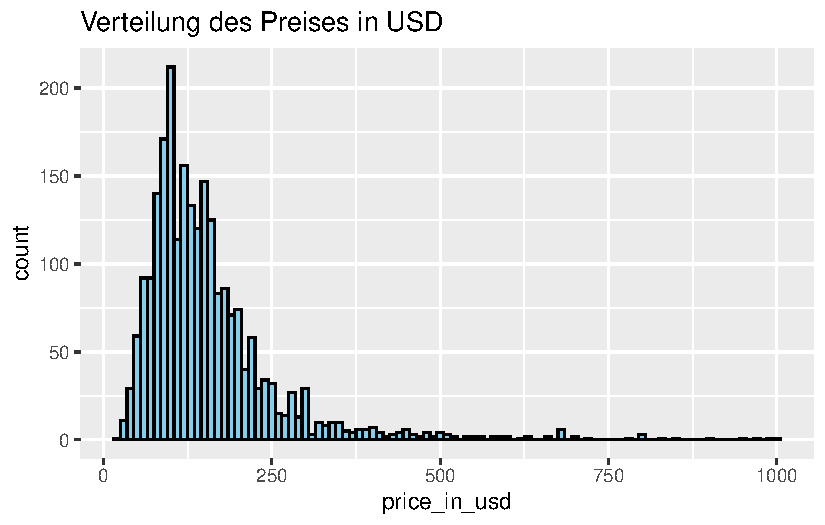
\includegraphics{main_files/figure-pdf/eda-1.pdf}

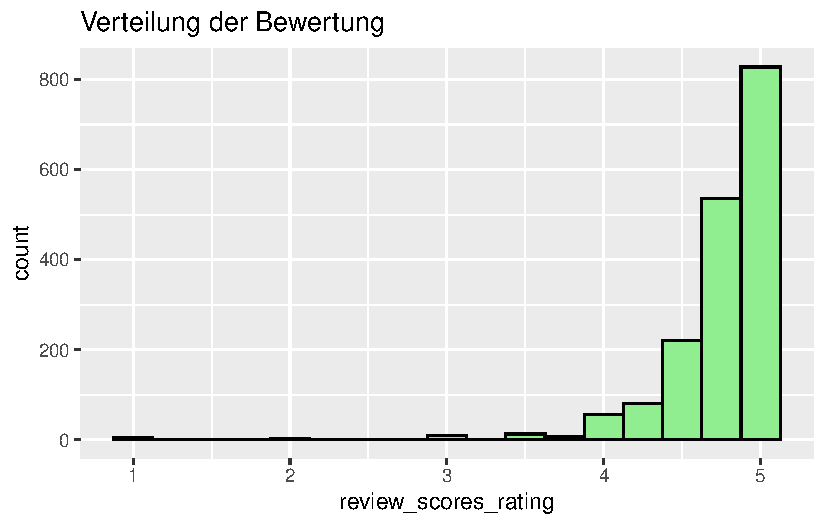
\includegraphics{main_files/figure-pdf/eda-2.pdf}

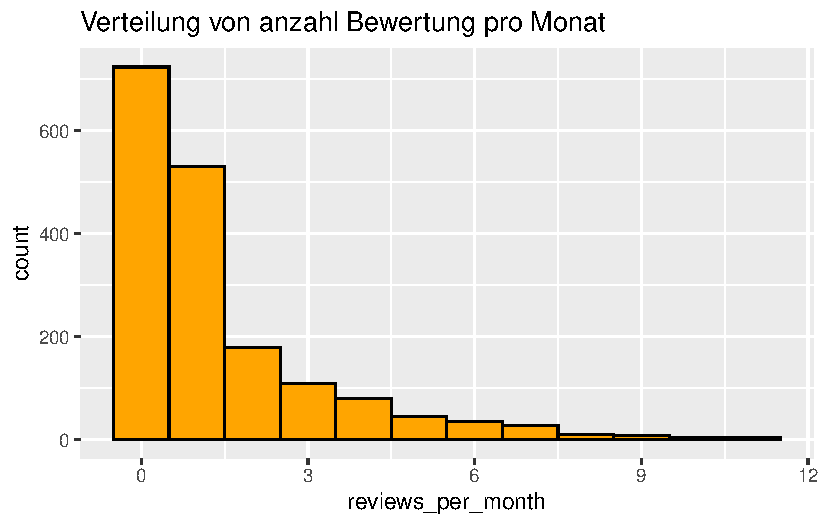
\includegraphics{main_files/figure-pdf/eda-3.pdf}

\hypertarget{datenanalyse-informationen-zur-datenstruktur-organisation-und-zu-den-fuxfcr-die-analyse-verwendeten-methoden}{%
\section{5. Datenanalyse (Informationen zur Datenstruktur, Organisation
und zu den für die Analyse verwendeten
Methoden)}\label{datenanalyse-informationen-zur-datenstruktur-organisation-und-zu-den-fuxfcr-die-analyse-verwendeten-methoden}}

\emph{Data analysis {[}2pt{]} Cedric / Jovan}

\emph{Are data attributes clear and obvious discussed? {[}1pt{]}}

\emph{Are adequate EDA methodologies used for data analysis? {[}1pt{]}}

Die bereinigten Datensets der verschiedenen Orten sind alle gleich
aufgebaut. Da wir den Preis der einzelnen Airbnb Apparment anschauen
möchten ist dies unser wichtigster Wert:

\begin{verbatim}
   Min. 1st Qu.  Median    Mean 3rd Qu.    Max. 
   20.0    95.0   133.0   157.8   185.0   999.0 
\end{verbatim}

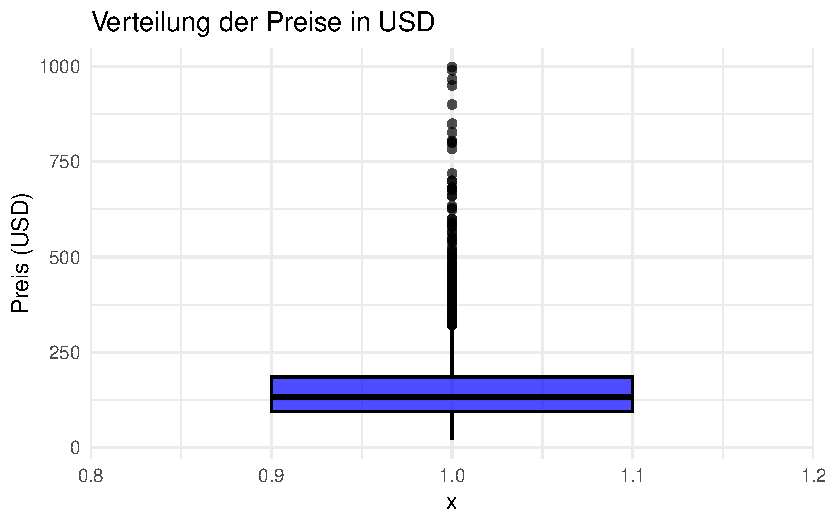
\includegraphics{main_files/figure-pdf/unnamed-chunk-5-1.pdf}

\begin{verbatim}
List of 3
 $ axis.title.x: list()
  ..- attr(*, "class")= chr [1:2] "element_blank" "element"
 $ axis.text.x : list()
  ..- attr(*, "class")= chr [1:2] "element_blank" "element"
 $ axis.ticks.x: list()
  ..- attr(*, "class")= chr [1:2] "element_blank" "element"
 - attr(*, "class")= chr [1:2] "theme" "gg"
 - attr(*, "complete")= logi FALSE
 - attr(*, "validate")= logi TRUE
\end{verbatim}

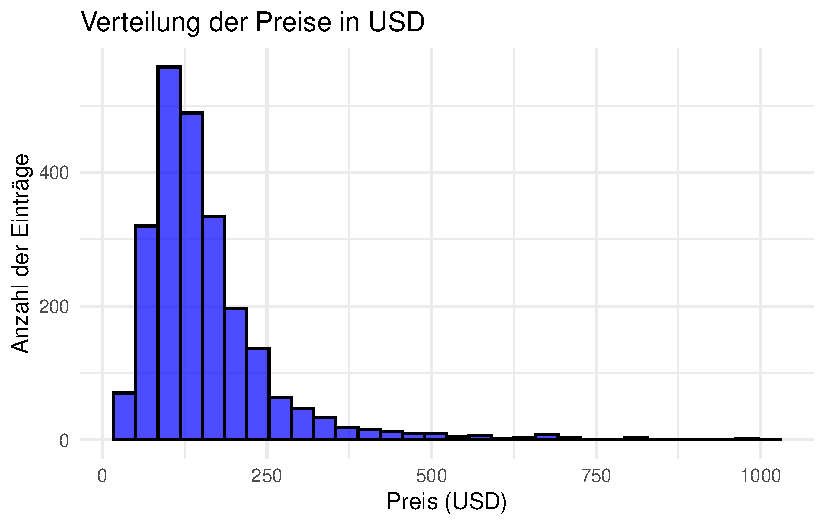
\includegraphics{main_files/figure-pdf/unnamed-chunk-5-2.pdf}

Nun ist stellt sich die Frage welche anderen Eigenschaften die grösste
Auswirkung auf den Preis haben. Dazu gilt es herauszufinden wie die
Korrelationen zwischen dem Preis pro USD und den anderen Attributen
sind:

\begin{verbatim}
                                          id 
                                -0.051733794 
                                   scrape_id 
                                          NA 
                                last_scraped 
                                 0.323817084 
                                     host_id 
                                -0.034408421 
                                  host_since 
                                -0.075722239 
                         host_listings_count 
                                -0.048121517 
                   host_total_listings_count 
                                -0.030748894 
                                    latitude 
                                -0.096602270 
                                   longitude 
                                 0.048817534 
                                accommodates 
                                 0.503562791 
                                        beds 
                                 0.419758800 
                              minimum_nights 
                                -0.100413698 
                              maximum_nights 
                                 0.078865097 
                      minimum_minimum_nights 
                                -0.045297000 
                      maximum_minimum_nights 
                                -0.024775869 
                      minimum_maximum_nights 
                                 0.100345512 
                      maximum_maximum_nights 
                                 0.041970938 
                      minimum_nights_avg_ntm 
                                -0.022747969 
                      maximum_nights_avg_ntm 
                                 0.042085419 
                             availability_30 
                                 0.103389623 
                             availability_60 
                                 0.112909276 
                             availability_90 
                                 0.110224160 
                            availability_365 
                                 0.130285779 
                       calendar_last_scraped 
                                 0.323817084 
                           number_of_reviews 
                                 0.003813291 
                       number_of_reviews_ltm 
                                -0.016722222 
                      number_of_reviews_l30d 
                                -0.021028955 
                                first_review 
                                -0.053134782 
                                 last_review 
                                 0.039951229 
                        review_scores_rating 
                                 0.057822255 
                      review_scores_accuracy 
                                 0.023426798 
                   review_scores_cleanliness 
                                 0.125133364 
                       review_scores_checkin 
                                 0.020947515 
                 review_scores_communication 
                                 0.006917651 
                      review_scores_location 
                                 0.091844483 
                         review_scores_value 
                                -0.008147618 
              calculated_host_listings_count 
                                -0.034790038 
 calculated_host_listings_count_entire_homes 
                                -0.026939926 
calculated_host_listings_count_private_rooms 
                                -0.116312035 
 calculated_host_listings_count_shared_rooms 
                                -0.026939558 
                           reviews_per_month 
                                -0.022824153 
               host_response_rate_in_percent 
                                 0.030119785 
             host_acceptance_rate_in_percent 
                                 0.042059103 
                                price_in_usd 
                                 1.000000000 
\end{verbatim}

Die Korrelationen der verschiedenen Variablen mit dem Preis
(\textbf{\texttt{price\_in\_usd}}) im Datensatz können wichtige
Einsichten bieten, welche Faktoren den Preis beeinflussen. Hier ist eine
Analyse der signifikanten positiven und negativen Korrelationen:

\hypertarget{positive-korrelationen}{%
\subsection{\texorpdfstring{\textbf{Positive
Korrelationen:}}{Positive Korrelationen:}}\label{positive-korrelationen}}

\begin{enumerate}
\def\labelenumi{\arabic{enumi}.}
\item
  \textbf{accommodates} (0.449): Es besteht eine moderate positive
  Korrelation zwischen der Anzahl der Gäste, die eine Unterkunft
  aufnehmen kann, und dem Preis. Dies deutet darauf hin, dass grössere
  Unterkünfte, die mehr Gäste beherbergen können, in der Regel teurer
  sind.
\item
  \textbf{beds} (0.329): Eine ähnliche positive Korrelation gibt es
  zwischen der Anzahl der Betten und dem Preis, was darauf hindeutet,
  dass mehr Betten oft höhere Preise bedeuten, was auch mit der Grösse
  der Unterkunft zusammenhängen kann.
\item
  \textbf{availability\_365} (0.157): Längere Verfügbarkeit im Laufe
  eines Jahres korreliert leicht positiv mit höheren Preisen. Dies
  könnte bedeuten, dass Unterkünfte, die seltener verfügbar sind, zu
  höheren Preisen angeboten werden.
\item
  \textbf{last\_scraped} (0.308), \textbf{calendar\_last\_scraped}
  (0.308): Diese Korrelationen deuten darauf hin, dass die Zeitpunkte
  der Datenerfassung mit den Preisänder
\end{enumerate}

\hypertarget{negative-korrelationen}{%
\subsection{\texorpdfstring{\textbf{Negative
Korrelationen:}}{Negative Korrelationen:}}\label{negative-korrelationen}}

\begin{enumerate}
\def\labelenumi{\arabic{enumi}.}
\item
  \textbf{latitude} (-0.097): Es gibt eine leichte negative Korrelation
  zwischen der geographischen Breite und dem Preis. Je weiter nördlich
  die Unterkunft liegt, desto geringer könnte der Preis sein, was auf
  regionale Preisunterschiede in der Stadt oder der Umgebung hinweisen
  könnte.
\item
  \textbf{minimum\_nights} (-0.053), \textbf{first\_review} (-0.053):
  Längere Mindestaufenthalte und frühere erste Bewertungen korrelieren
  leicht negativ mit dem Preis. Dies könnte darauf hinweisen, dass
  preisgünstigere Unterkünfte möglicherweise längere Aufenthalte
  erfordern oder schon länger auf dem Markt sind.
\item
  \textbf{calculated\_host\_listings\_count\_private\_rooms} (-0.103):
  Eine höhere Anzahl von Inseraten, die private Zimmer betreffen,
  korreliert leicht negativ mit dem Preis, was darauf hinweisen könnte,
  dass Gastgeber mit mehreren Einträgen möglicherweise günstigere Preise
  anbieten, um wettbewerbsfähig zu bleiben.
\end{enumerate}

\hypertarget{interpretation}{%
\subsection{\texorpdfstring{\textbf{Interpretation}}{Interpretation}}\label{interpretation}}

\begin{itemize}
\item
  \textbf{Hohe positive Korrelationen} zeigen an, dass mit zunehmender
  Kapazität und Verfügbarkeit der Unterkünfte der Preis steigt. Dies
  reflektiert die Marktlogik, dass grössere und häufiger verfügbare
  Unterkünfte als wertvoller angesehen werden.
\item
  \textbf{Negative Korrelationen} deuten darauf hin, dass bestimmte
  Faktoren wie die geografische Lage (nördlicher) oder die Politik
  längerer Mindestaufenthalte die Preise senken können. Dies könnte für
  Gäste attraktiv sein, die längerfristige Aufenthalte suchen oder
  flexibel in der Wahl der Region sind.
\end{itemize}

Diese Korrelationen sollten jedoch vorsichtig interpretiert werden, da
Korrelation nicht gleich Kausalität ist. Andere verborgene Variablen
könnten ebenfalls eine Rolle spielen, und die Effekte könnten durch
spezifische Marktbedingungen oder andere nicht berücksichtigte Faktoren
beeinflusst werden.

Um diese Korrelationen auch noch grafisch aufzuzeigen mit einer linearen
Regression.

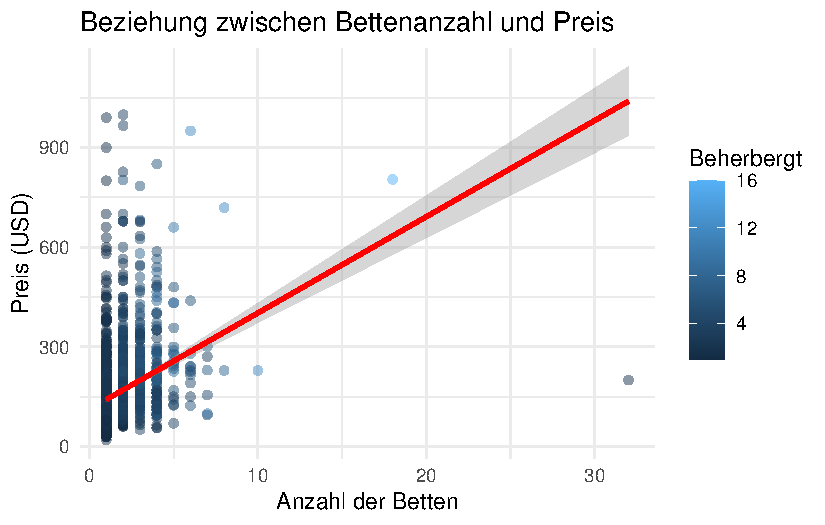
\includegraphics{main_files/figure-pdf/unnamed-chunk-7-1.pdf}

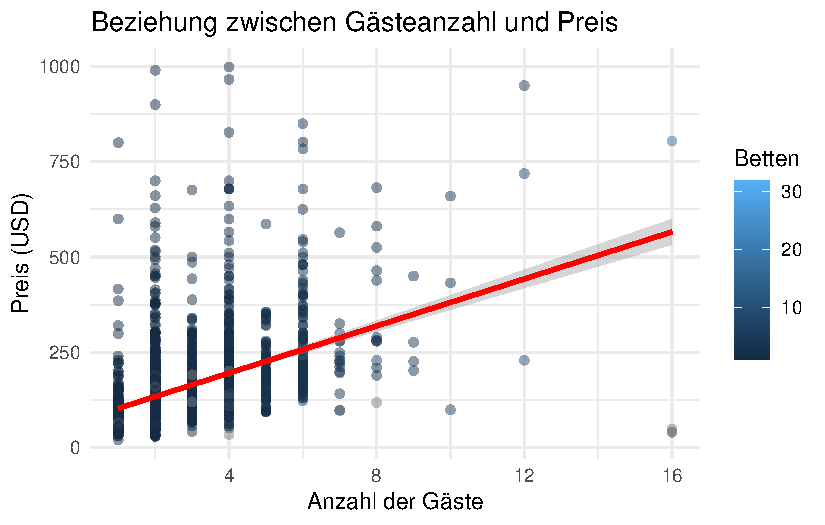
\includegraphics{main_files/figure-pdf/unnamed-chunk-7-2.pdf}

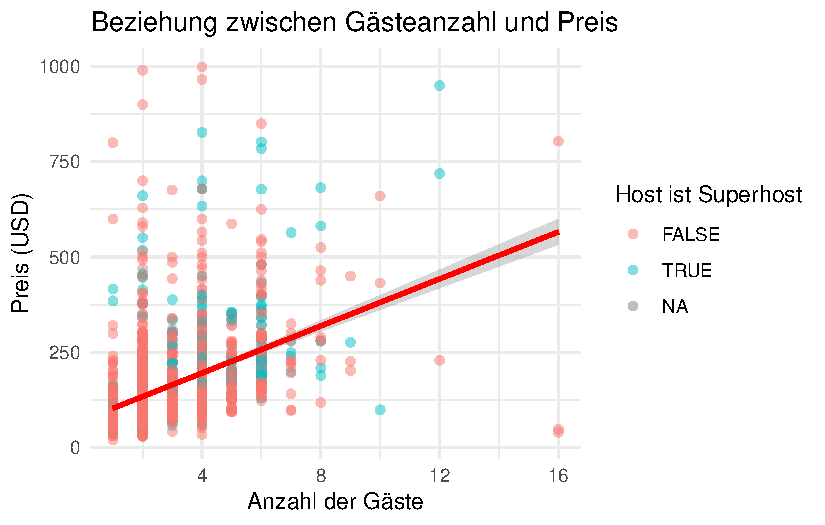
\includegraphics{main_files/figure-pdf/unnamed-chunk-7-3.pdf}

\emph{Die Analyse zeigt auf die irgendwie logische Korrelation zwischen
den Anzahl Gästen respektive Betten und den Preisen eines
AirBNBs\ldots{} Also je grösser das AirBNB desto mehr kostet es\ldots{}}

Gibt es noch andere Korrelationen welche nicht so klar ersichtlich sind?

Vielleicht sind die negativen Beziehungen spannender:

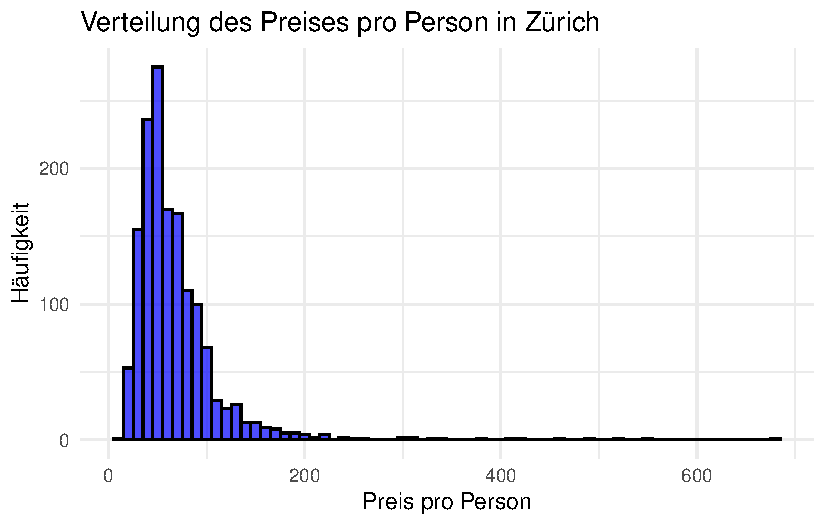
\includegraphics{main_files/figure-pdf/unnamed-chunk-8-1.pdf}

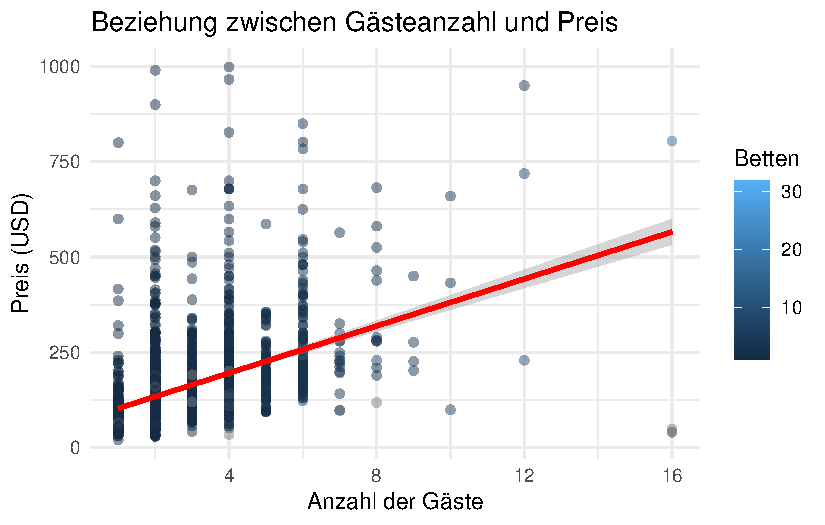
\includegraphics{main_files/figure-pdf/unnamed-chunk-8-2.pdf}

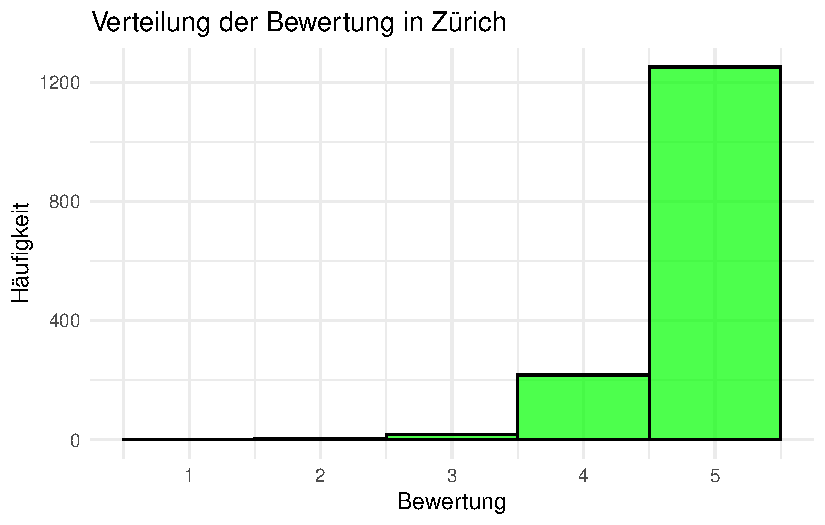
\includegraphics{main_files/figure-pdf/unnamed-chunk-8-3.pdf}

\emph{Sieht schon ein wenig besser aus - vorallem die Latitude. Wobei
auch hier ist es irgendwie klar. Je weiter weg das AirBNB von zentrum
weg ist desto günstiger ist die Wohnung\ldots{}}

\emph{Gibt es sonst noch irgendwelche Möglichkeiten den Preis
vorherauszusagen?}

Descriptive analysis {[}7pt{]}

\begin{enumerate}
\def\labelenumi{\arabic{enumi}.}
\tightlist
\item
  \textbf{Beschreibend (Descriptive)}: Deine Forschungsarbeit scheint
  beschreibende Analysen abzudecken, indem sie Merkmale von
  Airbnb-Unterkünften untersucht, die einen höheren Preis erzielen. Dies
  umfasst die Analyse der geografischen Lage, der Art der Unterkunft,
  der Anzahl der Zimmer und Bäder sowie der Verfügbarkeit von
  Annehmlichkeiten.
\end{enumerate}

\begin{itemize}
\item
  Was reasonable statistics used for data inspection and which
  attributes have been checked? {[}2pt{]}
\item
  Are the findings and statements qualitative? {[}3pt{]}
\item
  What are the conclusions of the findings? {[}2pt{]}
\end{itemize}

Predictive analysis {[}7pt{]}

\begin{enumerate}
\def\labelenumi{\arabic{enumi}.}
\tightlist
\item
  \textbf{Prädiktiv (Predictive)}: Um prädiktive Analysen einzubeziehen,
  könnte deine Fragestellung erweitert werden, um Vorhersagemodelle zu
  entwickeln, die den erzielbaren Preis basierend auf bestimmten
  Merkmalen der Unterkünfte prognostizieren. Dies könnte beispielsweise
  die Frage beinhalten: ``Welche Merkmale einer Airbnb-Unterkunft sind
  prädiktive Indikatoren für einen höheren Preis?''
\end{enumerate}

\begin{itemize}
\item
  Are the applied methods goal orientated? {[}2pt{]}
\item
  Were the applied methods qualitatively performed? {[}3pt{]}
\item
  What are the conclusions of the findings? {[}2pt{]}
\end{itemize}

Prescriptive analysis {[}7pt{]}

\begin{enumerate}
\def\labelenumi{\arabic{enumi}.}
\tightlist
\item
  \textbf{Präskriptiv (Prescriptive)}: Um präskriptive Analysen
  abzudecken, könnte die Forschung Empfehlungen entwickeln, wie
  Gastgeber ihre Unterkünfte modifizieren könnten, um die Attraktivität
  und den Preis zu maximieren. Die Frage könnte lauten: ``Welche
  Änderungen könnten Gastgeber vornehmen, um den Preis ihrer
  Airbnb-Unterkünfte zu maximieren?''
\end{enumerate}

\begin{itemize}
\item
  Is the applied method reasonable for the given problem? {[}2pt{]}
\item
  Were the applied methods qualitatively performed? {[}3pt{]}
\item
  What are the conclusions of the findings? {[}2pt{]}
\end{itemize}

\hypertarget{ergebnisse-statistische-ergebnisse-zahlen-diagramme}{%
\section{6. Ergebnisse (statistische Ergebnisse, Zahlen,
Diagramme)}\label{ergebnisse-statistische-ergebnisse-zahlen-diagramme}}

Conclusion {[}3pt{]}

\begin{itemize}
\item
  Are the initial BI problems reasonably discussed/solved? {[}2pt{]}
\item
  Are the obtained new insights of the data sets of good quality?
  {[}1pt{]}
\end{itemize}

\hypertarget{schlussfolgerung-beantwortung-der-frage}{%
\section{7. Schlussfolgerung (Beantwortung der
Frage)}\label{schlussfolgerung-beantwortung-der-frage}}

\hypertarget{referenzen}{%
\section{8. Referenzen}\label{referenzen}}

\begin{verbatim}
[1] 2
\end{verbatim}

\begin{verbatim}
[1] 4
\end{verbatim}

The \texttt{echo:\ false} option disables the printing of code (only
output is displayed).


% Can use something like this to put references on a page
% by themselves when using endfloat and the captionsoff option.
\ifCLASSOPTIONcaptionsoff
  \newpage
\fi

% trigger a \newpage just before the given reference
% number - used to balance the columns on the last page
% adjust value as needed - may need to be readjusted if
% the document is modified later
%\IEEEtriggeratref{8}
% The "triggered" command can be changed if desired:
%\IEEEtriggercmd{\enlargethispage{-5in}}

% Uncomment when use biblatex with style=ieee
%\renewcommand{\bibfont}{\footnotesize} % for IEEE bibfont size

\pagebreak[3]
% that's all folks
\end{document}

